%%%%%%%%%%%%%%%%%%%%%%%%%%%%%%%%%%%%%%%%
%% **** Start of file Quiz10.tex ***** %
%%%%%%%%%%%%%%%%%%%%%%%%%%%%%%%%%%%%%%%%

\documentclass[
    DIV=18,
    12pt,
    %paper=90mm:120mm,
    %pagesize,
    %twocolumn,
]{scrartcl}
%\usepackage[
%    paperwidth=90mm,
%    paperheight=120mm,
%    margin=0.10in,
%]{geometry}
\usepackage{amsmath}
\usepackage{booktabs}
\usepackage{enumitem}
\usepackage{multicol}
\usepackage{multirow}
\usepackage{pgfplots}
\usepackage{tabu}
\usepackage{tikz}
\usepackage{siunitx}
\usepackage{verbatim}

\begin{document}

\begin{center}
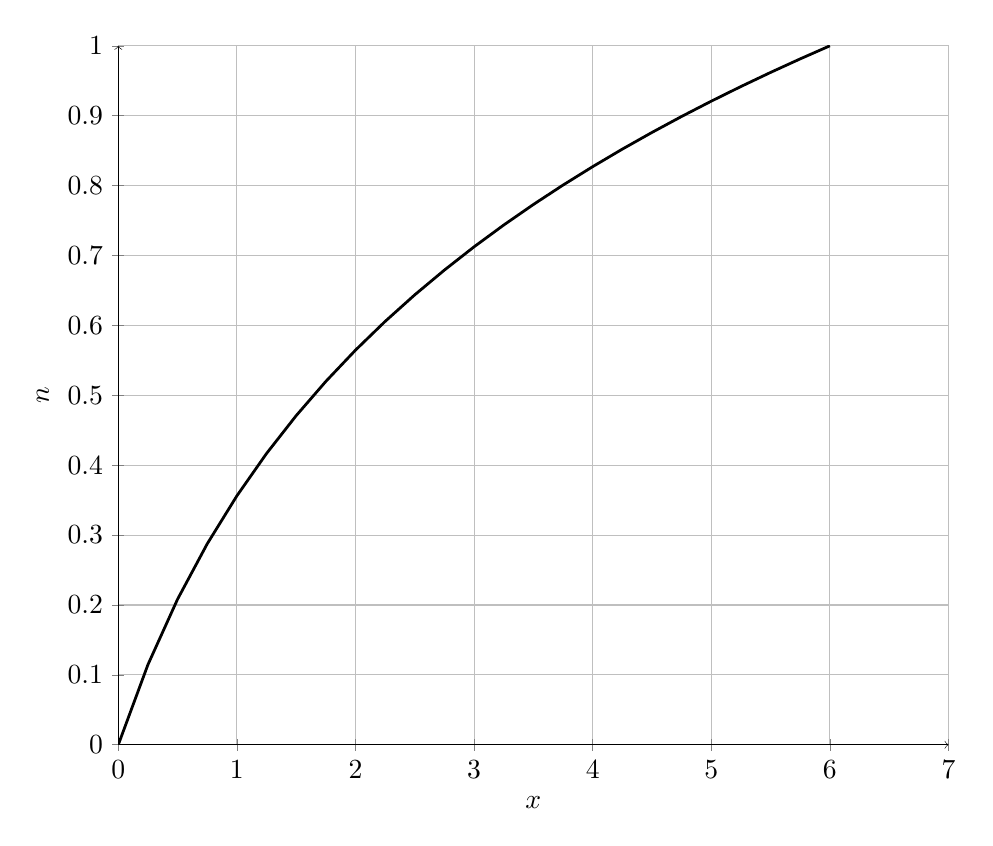
\begin{tikzpicture}
    \begin{axis}[
        axis y line=left,
        axis x line=bottom,
        axis line style={->},
        xlabel={$x$},
        %xtick={0.1,0.2,0.3,0.4,0.5,0.6,0.7,0.8,0.9,1.0},
        %minor x tick num=4,
        ylabel={$n$},
        %ytick={0,1,2,3,4,5,6,7,8,9,10},
        %minor y tick num=4,
        xmin=0,xmax=7,
        ymin=0,ymax=1,
        width=\linewidth,
        grid=major,
        very thin,
    ]
    %\addplot[line width=1pt,domain=0:1,samples=25] {11^x - 1};
    %\addplot[line width=1pt,domain=0:1,samples=25] {10^x - 1};
    %\addplot[line width=1pt,domain=0:1,samples=25] {9^x - 1};
    %\addplot[line width=1pt,domain=0:1,samples=25] {8^x - 1};
    \addplot[line width=1pt,domain=0:6,samples=25] {ln(x+1)/ln(7)};
    %\addplot[line width=1pt,domain=0:1,samples=25] {7^x - 1};
    %\addplot[line width=1pt,domain=0:1,samples=25] {ln(7) * 7^x};
    %\addplot[line width=1pt,domain=0:1,samples=25] {6^x - 1};
    %\addplot[line width=1pt,domain=0:1,samples=25] {5^x - 1};
    \end{axis}
\end{tikzpicture}
\end{center}

%

%% CRC Handbook of Chemistry and Physics 85th edition pp.2297
%%----------------------------------------------------------------------

\begin{comment}
\begin{itemize}
    \setlength{\itemindent}{3em}
    \setlength{\leftmargin}{0em}
    \setlength{\itemsep}{0em}
    \item[$t_m$:]   Melting point in \si{\degreeCelsius}
    \item[$t_b$:]   Normal boiling point in \si{\degreeCelsius}, at a pressure of \SI{101.325}{\kilo\pascal}.
    \item[$\Delta_{fus} H$:]    Enthalpy of fusion at the melting point in \si{\joule\per\gram}
    \item[$\rho_{25}$:]         Density at \SI{25}{\degreeCelsius} in \si{\gram\per\centi\meter\cubed}
    \item[$\alpha$:]            Coefficient of linear expansion at \SI{25}{\degreeCelsius} in \si{\per\kelvin} (the quantity listed is $10^5\times\alpha$)
    \item[$c_{p}$:]             Specific heat capacity at constant pressure at \SI{25}{\degreeCelsius} in \si{\joule\per\gram\per\kelvin}
    \item[$\lambda$:]           Thermal conductivity at \SI{27}{\degreeCelsius} in \si{\watt\per\centi\meter\per\kelvin}
\end{itemize}
\end{comment}

%\begin{comment}
\begin{center}
\begin{tabu}{ lSS SSS SSS }
    \toprule
    \multicolumn{1}{c}{Metal}
        & {Atomic}
        & {$t_m$}
        & {$t_b$}
        & {$\Delta_{fus} H$}
        & {$\rho_{25}$}
        & {$\alpha\times10^6$}
        & {$c_{p}$}
        & {$\lambda$} \\
    \multicolumn{1}{c}{(symbol)}
        & {weight}
        & {\si{\degreeCelsius}}
        & {\si{\degreeCelsius}}
        & {\si{\joule\per\gram}}
        & {\si{\gram\per\centi\meter\cubed}}
        & {\si{\per\kelvin}}
        & {\si{\joule\per\gram\per\kelvin}}
        & {\si{\watt\per\centi\meter\per\kelvin}} \\
    \midrule
    {Aluminum (Al)}
        & 26.98
        & 660.32
        & 2519
        & 399.9
        & 2.70
        & 23.1
        & 0.904
        & 2.37 \\
    {Copper (Cu)}
        & 63.55
        & 1084.62
        & 2502
        & 203.5
        & 8.86
        & 16.5
        & 0.384
        & 4.01 \\
    {Gold (Au)}
        & 196.97
        & 1062.18
        & 2856
        & 64.6
        & 19.3
        & 14.2
        & 0.129
        & 3.17 \\
    {Iron (Fe)}
        & 55.85
        & 1538
        & 2861
        & 247.3
        & 7.87
        & 11.8
        & 0.449
        & 0.802 \\
    {Lead (Pb)}
        & 207.20
        & 327.46
        & 1749
        & 23.1
        & 11.3
        & 28.9
        & 0.127
        & 0.353 \\
    {Mercury (Hg)}
        & 200.59
        & -38.83
        & 356.62
        & 11.4
        & 13.5336
        & 60.4
        & 0.139
        & 0.0834 \\
    {Neodymium (Nd)}
        &
        & 644
        &
        & 13.5
        & 20.2
        &
        &
        & 0.063 \\
    {Platinum (Pt)}
        & 195.08
        & 1768.2
        & 3825
        & 113.6
        & 21.5
        & 8.8
        & 0.133
        & 0.716 \\
    {Silver (Ag)}
        & 107.87
        & 961.78
        & 2162
        & 104.6
        & 10.5
        & 18.9
        & 0.235
        & 4.29 \\
    {Tin (Sn)}
        & 118.71
        & 231.93
        & 2602
        & 60.4
        & 7.26
        & 22.0
        & 0.227
        & 0.666 \\
    {Zinc (Zn}
        & 65.39
        & 419.53
        & 907
        & 108.1
        & 7.14
        & 30.2
        & 0.388
        & 1.16 \\
    \bottomrule
\end{tabu}
\end{center}
%\end{comment}


%\begin{comment}
\begin{center}
\begin{tabu}{ l SSSS }
    \toprule
    elements    & $T_m$
                & $T_b$
                & $L_f$
                & $L_v$ \\
                & \si{\degreeCelsius}
                & \si{\degreeCelsius}
                & \si{\kilo\joule\per\kilo\gram}
                & \si{\kilo\joule\per\kilo\gram} \\
    \midrule
    aluminum    & 660
                & 2519
                & 397
                & 10,900 \\
    argon       & -189
                & -186
                & 29.5
                & 161 \\
    bismuth     & 271
                & 1564
                & 54.0
                & 723 \\
    bromine (Br\textsubscript{2})
                & -7
                & 59
                & 132
                & 375 \\
    chlorine (Cl\textsubscript{2})
                & -102
                & -34
                & 181
                & 576 \\
    copper      & 1084
                & 2562
                & 209
                & 4730 \\
    gold        & 1064
                & 2856
                & 63.7
                & 1645 \\
    helium      & -272
                & -269
                & 3.45
                & 20.7 \\
    hydrogen (H\textsubscript{2})
                & -259
                & -253
                & 59.5
                & 445 \\
    iron        & 1538
                & 2861
                & 247
                & 6090 \\
    krypton     & -157
                & -153
                & 16.3
                & 108 \\
    lead        & 327
                & 1749
                & 23.0
                & 866 \\
    lithium     & 181
                & 1342
                & 432
                & 21,200 \\
    mercury     & -39
                & 357
                & 11.4
                & 295 \\
    neon        & -249
                & -246
                & 16.8
                & 84.8 \\
    nickel      & 1455
                & 2913
                & 298
                & 6430 \\
    nitrogen (N\textsubscript{2})
                & -210
                & -196
                & 25.3
                & 199 \\
    oxygen (O\textsubscript{2})
                & -219
                & -183
                & 13.7
                & 213 \\
    platinum    & 1768
                & 3825
                & 4.32
                & 99.5 \\
    plutonium   & 640
                & 3228
                & 11.6
                & 1370 \\
    silicon     & 1414
                & 3265
                & 1790
                & 12 800 \\
    silver      & 962
                & 2162
                & 105
                & 2390 \\
    sodium      & 98
                & 883
                & 113
                & 4240 \\
    sulfur      & 115
                & 445
                & 53.6
                & 1400 \\
    tin         & 231
                & 2602
                & 59.2
                & 2490 \\
    titanium    & 1668
                & 3287
                & 296
                & 8880 \\
    tungsten    & 3422
                & 5555
                & 285
                & 4390 \\
    uranium     & 1135
                & 4131
                & 38.4
                & 1750 \\
    zinc        & 420
                & 907
                & 112
                & 1890 \\
    \bottomrule
\end{tabu}
\end{center}
%\end{comment}

\begin{comment}
\begin{center}
\begin{tabu}{ l SSSS }
    \toprule
    compounds   & $T_m$
                & $T_b$
                & $L_f$
                & $L_v$ \\
                & \si{\degreeCelsius}
                & \si{\degreeCelsius}
                & \si{\kilo\joule\per\kilo\gram}
                & \si{\kilo\joule\per\kilo\gram} \\
    \midrule
    %compounds   Tm (℃)  Tb (℃)  Lf (kJ/kg)  Lv (kJ/kg)
    alcohol, ethyl      & -130
                        & 78
                        &
                        & \\
    alcohol, methyl     & -97
                        & 64.7
                        &
                        & \\
    ammonia             & -77.7
                        & -33.3
                        &
                        & \\
    butane              & -138.4
                        & -0.5
                        & 80.2
                        & \\
    carbon dioxide      &
                        &
                        & 571
                        & 205 \\
    ethane              & -172
                        & -89
                        & 95.1
                        & \\
    freon 12, -30       & -158
                        & -29.8
                        &
                        & 166.2 \\
    freon 12, 0         & -158
                        & -29.8
                        &
                        & 152.8 \\
    freon 12, 30        & -158
                        & -29.8
                        &
                        & 136.3 \\
    methane             & -182
                        & -164
                        & 58.4
                        & 112 \\
    propane             & -188
                        & -44.5
                        & 80.1
                        & \\
    water, 0            & 0
                        & 100
                        & 334
                        & 2501 \\
    water, 25           & 0
                        & 100
                        &
                        & 2441 \\
    water, 100          & 0
                        & 100
                        &
                        & 2258 \\
    wax, beeswax        & 62
                        &
                        &
                        & \\
    \bottomrule
\end{tabu}
\end{center}
\end{comment}


\begin{comment}
\begin{center}
\begin{tabu}{ l SSSS }
    \toprule
    foods       & $T_m$
                & $T_b$
                & $L_f$
                & $L_v$ \\
                & \si{\degreeCelsius}
                & \si{\degreeCelsius}
                & \si{\kilo\joule\per\kilo\gram}
                & \si{\kilo\joule\per\kilo\gram} \\
    \midrule
    %foods   Tm (℃)  Tb (℃)  Lf (kJ/kg)  Lv (kJ/kg)
    butter              & 32--35
                        &
                        &
                        & \\
    lard                & 41
                        &
                        &
                        & \\
    margarine, table    & 34--37
                        &
                        &
                        & \\
    margarine, bakery   & 38--43
                        &
                        &
                        & \\
    oil, cocoa butter   & 34
                        &
                        &
                        & \\
    oil, coconut        & 24
                        &
                        &
                        & \\
    %oil, corn           & \SI{−20}? −15?
    oil, olive          & -6
                        &
                        &
                        & \\
    %oil, palm   ~35
    oil, peanut         & 3
                        &
                        &
                        & \\
    oil, soya   −16? −13?
    shortening, vegetable   44~50
    sugar, fructose     & 104
    sugar, glucose  146
    sugar, sucrose  186
    \bottomrule
\end{tabu}
\end{center}
\end{comment}

\pagebreak

\endinput



\end{document}


